\section{Optimización intertemporal y la aversión al cambio}
\subsection{Introducción al modelo de consumo intertemporal}
El economista y estadístico \textbf{Irving Fisher}\marginnote{\textbf{Irving Fisher 1867-1947:} Economista y estadístico estadounidense reconocido por sus avances en la teoría económica (Ecuación de Fisher, hipótesis de Fisher, teorema de separabilidad de Fisher...).} desarrolló en gran parte uno de los modelos más influyentes en como entendemos que se toman las decisiones de consumo a lo largo del tiempo. Para esto tenemos que pensar en un individuo que se detiene a pensar en el presente cuanto consumirá ahora y cuanto consumirá en cada período en el futuro. 

Este modelo considera un consumidor racional que enfrenta restricciones a su consumo a lo largo del tiempo. Una simplificación que haremos para presentar el modelo será que el consumidor solo vive dos períodos. 

Uno de los factores más importantes de este modelo es la capacidad de que el individuo ahorre y contraiga deuda. Es la manera en que el consumidor podrá transportar dinero del presente al futuro (ahorro) o viceversa del futuro al presente (deuda).

Partiremos armando intuitivamente la restricción de cada período para así juntarlas y obtener lo que llamaremos una \textbf{restricción intertemporal}.

\subsection{Restricción intertemporal}
\marginnote{\textbf{Restricción intertemporal:} Restricción resultante de consumir con un ingresos finitos transferibles entre períodos de tiempo}
El individuo representativo partirá consumiendo en el período uno ($c_1$), para financiar su consumo recibirá un ingreso $y_1$. Lo primero que podemos sacar es que el individuo va a estar restringido pues todo consumo debe estar respaldado por ingreso, $y_1 \geq c_1$. Aquí vamos a añadir otro factor a la mezcla, el individuo podrá ahorrar o endeudarse. Este factor ahorro/deuda lo denotaremos por $s$, será $>0$ cuando se trate de ahorro y será $<0$ cuando sea deuda.

Con esto ya podemos definir la restricción en el primer período como la ecuación \ref{eq: rest 1}.
\begin{equation}
    y_1 = c_1+s \label{eq: rest 1}
\end{equation}

En el segundo período la restricción seguirá la misma lógica, lo que hay que considerar adicionalmente es que hay una tasa de interés ($r$) de por medio para cuando uno ahorra o se endeuda. Por lo que los ingresos $y$ en un período, se convertirán en $y(1+r)$ en el siguiente período.

La restricción del segundo período puede ser descrita como la ecuación \ref{eq: rest 2}.
\begin{equation}
    y_2 = c_2 - s(1+r) \label{eq: rest 2}
\end{equation}

Teniendo las restricciones para los dos períodos podemos describir una restricción intertemporal combinandolas. Para esto reemplazamos $s$ de \ref{eq: rest 1} en \ref{eq: rest 2}.
\begin{equation*}
    y_2 = c_2 - (1+r)(y_1-c_1) 
\end{equation*}

Reordenando podemos encontrar dos expresiones útiles que representan la misma restricción, las dos significan que todo el consumo tiene que ser financiado por ingreso. 

La expresión \ref{eq: valor futuro} está ordenada de forma que los ingresos presentes sean traídos a \textbf{valor futuro},\marginnote{\textbf{Valor futuro:} El valor que tendrá cierta monto en un período futuro dadas las oportunidades de ahorro/inversión.}[-4cm]mientras que \ref{eq: valor presente} está expresado de forma en que los ingresos futuros sean traídos a \textbf{valor presente}.\marginnote{\textbf{Valor presente:} El valor que tiene cierto monto en el futuro traído a lo que valdría hoy dadas las oportunidades de ahorro/inversión.}
\begin{align}
    y_1(1+r) + y_2 &= c_1(1+r) + c_2 \label{eq: valor futuro} \\
    \quad & \quad \notag\\
    y_1 + \frac{y_2}{1+r} &= c_1 + \frac{y_2}{1+r} \label{eq: valor presente}
\end{align}

Esta restricción intertemporal puede ser graficada tal como una restricción presupuestaria (Véase la figura \ref{fig: restricción intertemporal}). De esta recta el consumidor decidirá en qué punto maximiza su utilidad, de este punto sabremos si el consumidor se está endeudando o ahorrando. 
\begin{figure}
    \centering
    \caption{Restricción intertemporal}
    \includegraphics[width=\textwidth]{Figuras/CI Restricción intertemporal.jpeg}
    \label{fig: restricción intertemporal}
\end{figure}

El punto en que el consumidor elija para maximizar su utilidad podrá ser utilizado para ver si está ahorrando o endeudándose. Es directo ver que si $c_1>y_1$ implica que $s<0$, es decir se está contrayendo deuda para financiar el consumo presente. Para financiar esa deuda el consumidor estará obligado en el futuro a que $c_2<y_2$ pues cierta parte va a ser usada para pagar la deuda. Tanto este caso como el caso en que el individuo ahorra se pueden ver en la figura \ref{fig: restricción intertemporal}.

Por otro lado es relevante entender por qué el consumo máximo de $c_2$ en la figura está en valor futuro, mientras que el consumo máximo $c_1$ está en valor presente. 

Un caso que se verá más adelante son las restricciones de liquidez, es decir cuando la tasa a la que uno se endeuda es más alta a la cual uno ahorra.\footnote{Un caso extremo en que la tasa a la que uno se endeuda tiene a infinito llevará inevitablemente a este consumidor racional a comportarse como un consumidor keynesiano.} 

\subsection{El consumidor}

El consumidor racional en esta ocasión maximizará utilidad mediante consumo en dos períodos. Tendrá una función de utilidad para un período $i$ tal que $u'(c_i)>0$ y $u''(c_2)<0$, es decir, es decir cada unidad de consumo tendrá efectos positivos sobre su utilidad pero a rendimientos decrecientes. La concavidad de la función de utilidad se puede interpretar como que el individuo es saciable y esa es una de las razones por las que preferirá suavizar su consumo a lo largo del tiempo

La utilidad entre estos dos períodos puede ser expresado simplemente como la suma entre $u(c_1)$ y $u(c_2)$ pero añadiremos un matiz más. El consumidor tendrá una preferencia por el consumo en el presente por sobre el consumo en futuro. Para modelar esta preferencia añadiremos una \textbf{tasa de impaciencia} que descontará el consumo en futuro. Podemos expresar la función de utilidad entre los dos períodos en la ecuación \ref{eq: ut intertemporal}.
\begin{equation}
    U(c_1,c_2) = u(c_1) + \frac{1}{1+\rho} u(c_2) \label{eq: ut intertemporal}
\end{equation}
Por conveniencia podemos hacer un cambio de variable y definir $\beta = \frac{1}{1+\rho}$. 

\subsection{El problema y resolución del consumidor}
Ahora podemos plantear el problema del consumidor como una función a maximizar sujeto a una restricción.
\begin{align*}
        \max_{c_1,c_2} & \quad \Bigl\{ u(c_1) + \beta u(c_2) \Bigr\} \\ s.a.& \quad  y_1 + \frac{y_2}{1+r} = c_1 + \frac{c_2}{1+r}
\end{align*}
Para resolver este problema definimos el lagrangeano y derivamos las condiciones de primer orden. 
\begin{align}
        \mathcal{L}:& u(c_1) + \beta u(c_2) + \lambda \left( y_1 + \frac{y_2}{1+r} - c_1 - \frac{c_2}{1+r} \right) \notag \\
        \text{CPO:} \quad & \frac{\partial \mathcal{L}}{\partial c_1} = u'(c_1) - \lambda = 0 \notag \\
        &\frac{\partial \mathcal{L}}{\partial c_2} = \beta u'(c_2) - \frac{\lambda}{1+r} = 0 \notag \\
        & \lambda = \lambda \longrightarrow u'(c_1) = \left( \frac{1}{1+\rho} \right) u'(c_2)(1+r) \notag \\
        &  \frac{u'(c_1)}{u'(c_2)} = \frac{1+r}{1+\rho} \label{eq: perfil del consumidor}
    \end{align}
El resultado de la optimización va a ser la expresión \ref{eq: perfil del consumidor}, conocida como la \textbf{ecuación de Euler del consumo}. Esta ecuación se puede interpretar como el perfil del consumidor, como se ajusta el consumo en cada período dada la tasa de interés y la tasa de impaciencia. 

Por ejemplo, un aumento de la tasa de interés tiene un efecto positivo sobre el consumo futuro en relación con el consumo presente. Que el consumo presente disminuya implica que la utilidad marginal del consumo presente aumente\footnote{Esto debido a los rendimientos decrecientes de la utilidad del consumo.} esto tendría el efecto contrario en el consumo futuro. 

\subsection{Tasa de interés y tasa de impaciencia}

Hasta ahora solo hemos mencionado estas tasas como factores que considera el consumidor para mover su dinero entre períodos. Lo primero que se busca entender es que son fuerzas contrarias, una lleva consumo del presente al futuro y la otra del futuro al presente. Una forma más formal de empezar a entender estas fuerzas es como precios relativos de cada consumo

El precio relativo de consumo presente en relación al consumo futuro es la tasa de interés, puesto que el dinero que no se gaste en el presente será $(1+r)$ más valioso en el futuro. En el perfil del consumidor \ref{eq: perfil del consumidor} un aumento de un $1\%$ en la tasa de interés tendrá un efecto de un $1\%$ en el consumo futuro en relación al consumo presente.

A continuación veremos un caso en que los cambios en los precios relativos del consumo en cada período no tienen una relación 1 a 1 con los ajustes. Es decir que la elasticidad entre estas variables no va a ser igual a 1.

\subsection{Funciones de utilidad con aversión al riesgo}

Un caso especial y muy utilizado para describir el consumo de agentes en la economía es el uso de funciones de utilidad que incluyan aversión al riesgo. Las funciones de aversión relativa al riesgo constante (CRRA) incluyen el factor aversión al riesgo como una variable $\sigma$ que tendrá un efecto sobre la magnitud de los ajustes ante cambios en las variables exógenas (Como la tasa de interés por ejemplo). 

Un función de utilidad CRRA se puede describir como la expresión \ref{eq: CRRA}.
\begin{equation}
    u(c)= \left\{ \begin{array}{lcc} \frac{c^{1-\sigma}-1}{1-\sigma} & \text{si} & \sigma >0,\sigma \neq 1 \\ \\ \ln{(c)} & \text{si} & \sigma = 1 \end{array} \right. \label{eq: CRRA}
\end{equation}

De la cual si resolvemos como hicimos en el consumo intermtemporal anterior llegaremos a una ecuación de Euler del consumo (expresada en \ref{eq: perfil con aversión al riesgo}). De aquí podemos definir la \textbf{elasticidad intertemporal de sustitución} como el cambio porcentual en la relación marginal de consumo 1 y 2 para un cambio del $1\%$ en el precio relativo del consumo en 1 (tasa de interés). 
\begin{equation}
    \left( \frac{u'(c_1)}{u'(c_2)} \right) ^\sigma=  \frac{1+r}{1+\rho}  \label{eq: perfil con aversión al riesgo}
\end{equation}

La elasticidad intertemporal de sustitución describe la magnitud en que el consumo presente y futuro se ajustan ante un cambio en las condiciones (tasa de interés e impaciencia). 
\begin{equation}
    \text{EIS} = - \frac{\partial \ln (u'(c_1)/u'(c_2))}{\partial \ln (1+r)} = \frac{1}{\sigma}
\end{equation}

Mientras mayor sea la aversión al riesgo ($\sigma$) el consumidor responderá en menor medida a cambios en estas variables. Es decir, un aumento de $1\%$ en el precio relativo del consumo presente en relación al consumo futuro tendrá un efecto $1/\sigma$ en la relación de consumo futuro y consumo presente.

Mientras mayor sea la $\sigma$ mayor será la aversión al riesgo, representado por una curva más cóncava. 

\subsection{Restricciones de liquidez}

Hasta ahora se ha asumido que la tasa a la que un individuo ahorra ($r$) y se endeuda ($r^*$) es la misma. Un acercamiento más realista es que la tasa que paga un deudor es mayor a la tasa que consigue alguien por ahorrar. 

Cuando hablamos de \textbf{restricciones de liquidez} específicamente nos referimos a restricciones al endeudamiento. Este margen puede deberse a que la tasa de endeudamiento considera un premio por riesgo cuando hay probabilidad de impago. Mercados financieros menos robustos, los cuales suelen estar presentes en países menos desarrollados suelen estar sujetos a mayores restricciones de liquidez, lo cual deriva en muchas implicancias macro y microeconómicas.\footnote{Efectos sobre inversión y aplificación del ciclo económico, racionamiento del crédito, ineficiencias que llevan a perpetuar la desigualdad, etc\ldots}

\begin{figure}[t]
    \centering
    \caption{Restricciones de liquidez y perdida de bienestar ahorradores y deudores}
    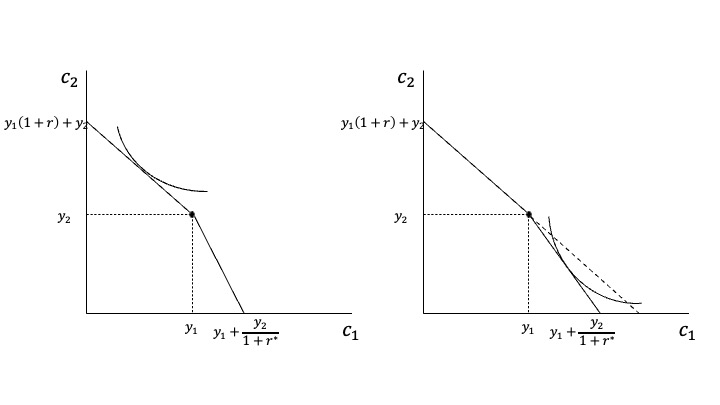
\includegraphics[width=\textwidth]{Figuras/CI Restricciones de liquidez.jpeg}
    \label{fig: Restricciones liquidez bienestar}
\end{figure}

Podemos ver los efectos en el bienestar de un consumidor bajo restricciones de liquidez en dos casos. Uno en el cual el consumidor prefiere ahorrar, en este caso se dice que la restricción no está activa puesto que las restricciones de liquidez solo afectan a la tasa de endeudamiento (Figura \ref{fig: Restricciones liquidez bienestar}). El caso en que el individuo preferiría endeudarse, en estas condiciones la restricción está activa, el punto que maximizaba el bienestar ya no es factible y por tanto hay una perdida en cuanto a utilidad. 

Es fácil ver que las restricciones tienen efectos negativos (o nulos) en el bienestar de las personas pues reduce la cantidad de opciones factibles en las que maximizar utilidad. 